% ---
% 07. Casa de José Veríssimo Alves na rua do Sangradouro
% ---

\afterpage{
\begin{a3paisagem}
\begin{figure}[!h]
\centering
\caption{Representação da casa de nº 24 sita a rua do Sangradouro com projecto de mais um pavimento (1920). }
\includegraphics[width=1\textwidth]{8-anexos/plantas/01-1distrito/15-sangradouro/sangradouro-joseverissimoalves-1920.jpg}{\footnotesize \par  \textbf{Fonte:} \textbf{BR BAAHMS}, Fundo ``Intendência'', Série ``Processos de Licenciamento de Reforma e Ampliação de Edificações'', Subsérie ``Requerimentos e Plantas -- Brotas'', caixa 15. \par Projeto de Custódio Bandeira (1920). A casa de José Veríssimo Alves é uma das poucas a permanecer de pé neste logradouro. }
\label{fig:joseverissimo1920}
\end{figure}
\end{a3paisagem}
}

% ---
% 08. Casa de José Veríssimo Alves ainda de pé
% ---

\afterpage{
\begin{figure}[!h]
\centering
\caption{Antiga casa de José Veríssimo Alves, na rua do Sangradouro (2017). }
\includegraphics[width=1\textwidth]{8-anexos/plantas/01-1distrito/15-sangradouro/sangradouro-joseverissimoalves-2019n169.jpg}{\footnotesize \par   \textbf{Fonte:} Google Maps. }
\label{fig:joseverissimo2017}
\end{figure}
}

% ---
% 09. Casa de Domingos Gonçalves Cavalheiros na rua do Castro Neves, ainda de pé
% ---

\afterpage{
\begin{a3paisagem}
\begin{figure}[!htp]
	\caption{Casa de Domingos Gonçalves Cavalheiro, na rua do Castro Neves, em dois tempos}
	\centering
		\begin{subfigure}[t]{0.4\textwidth}
			\includegraphics[width=1\textwidth]{8-anexos/plantas/01-1distrito/16-castroneves/castroneves240-domingosgoncalvescavalheiro-1927.jpg}
			\caption{\footnotesize Projeto de Pedro Jayme David (1927). \textbf{Fonte:} \textbf{BR BAAHMS}, Fundo ``Intendência'', Série ``Processos de Licenciamento de Reforma e Ampliação de Edificações'', Subsérie ``Requerimentos e Plantas -- Brotas'', caixa 16. }
			\label{fig:domingosgoncalvescavalheiro-1927}
		\end{subfigure}
		\
		\begin{subfigure}[t]{0.4\textwidth}
			\includegraphics[width=1\textwidth]{8-anexos/plantas/01-1distrito/16-castroneves/castroneves240-domingosgoncalvescavalheiro-2017.jpg} 
			\caption{\footnotesize  O mesmo imóvel em 2017. \textbf{Fonte:} Google Maps. }
			\label{fig:domingosgoncalvescavalheiro-2017}
		\end{subfigure}
	\label{fig:domingosgoncalvescavalheiro}
\end{figure}
\end{a3paisagem}
}

% ---
% 10. Duas casas de Maria Rosa Vianna Ferraz na rua do Castro Neves
% ---

\afterpage{
\begin{a3paisagem}
\begin{figure}[!h]
\centering
\caption{Projecto para modificação das fachadas dos predios nº 81 e 83 a rua Castro Neves districto de Brotas (1929). }
\includegraphics[height=0.9\textheight]{8-anexos/plantas/01-1distrito/16-castroneves/mariarosaviannaferraz-83e81-1929.jpg}{\footnotesize \par  Projeto de Lycerio Alfredo Schreiner. \textbf{Fonte:} \textbf{BR BAAHMS}, Fundo ``Intendência'', Série ``Processos de Licenciamento de Reforma e Ampliação de Edificações'', Subsérie ``Requerimentos e Plantas -- Brotas'', caixa 16. Uma das duas casas de Maria Rosa Vianna Ferraz permanece de pé. }
\label{fig:mariarosaviannaferraz1929}
\end{figure}
\end{a3paisagem}
}

% ---
% 11. Casa de Maria Rosa Vianna Ferraz ainda de pé
% ---

\afterpage{
\begin{figure}[!h]
\centering
\caption{Antiga casa de Maria Rosa Vianna Ferraz, na rua do Castro Neves (2017). }
\includegraphics[height=0.9\textheight]{8-anexos/plantas/01-1distrito/16-castroneves/mariarosaviannaferraz-83e81-2017.jpg}{\footnotesize \par \textbf{Fonte:} Google Maps. }
\label{fig:mariarosaviannaferraz2017}
\end{figure}
}

% ---
% 12. Casa de Edmundo Guimarães na ladeira dos Galés
% ---

\afterpage{
\begin{a3paisagem}
\begin{figure}[!h]
\centering
\caption{Projecto para construção do 1ª andar do predio á Ladeira dos Galés nº 16. Propriedade do Illmº Snr. Edmundo Guimarães. Districto de Brotas (1930) }
\includegraphics[width=1\textwidth]{8-anexos/plantas/01-1distrito/12-gales/ladeiradosgales-edmundoguimaraes-casa.jpg}{\footnotesize \par  Projeto de Rossi Baptista (1930). \textbf{Fonte:} \textbf{BR BAAHMS}, Fundo ``Intendência'', Série ``Processos de Licenciamento de Reforma e Ampliação de Edificações'', Subsérie ``Requerimentos e Plantas -- Brotas'', caixa 12. Esta casa de Edmundo Guimarães permanece de pé. }
\label{fig:edmundoguimaraes1930}
\end{figure}
\end{a3paisagem}
}

% ---
% 13. Casa de Edmundo Guimarães ainda de pé
% ---

\afterpage{
\begin{figure}[!h]
\centering
\caption{Antiga casa de Edmundo Guimarães na ladeira dos Galés (2017)}
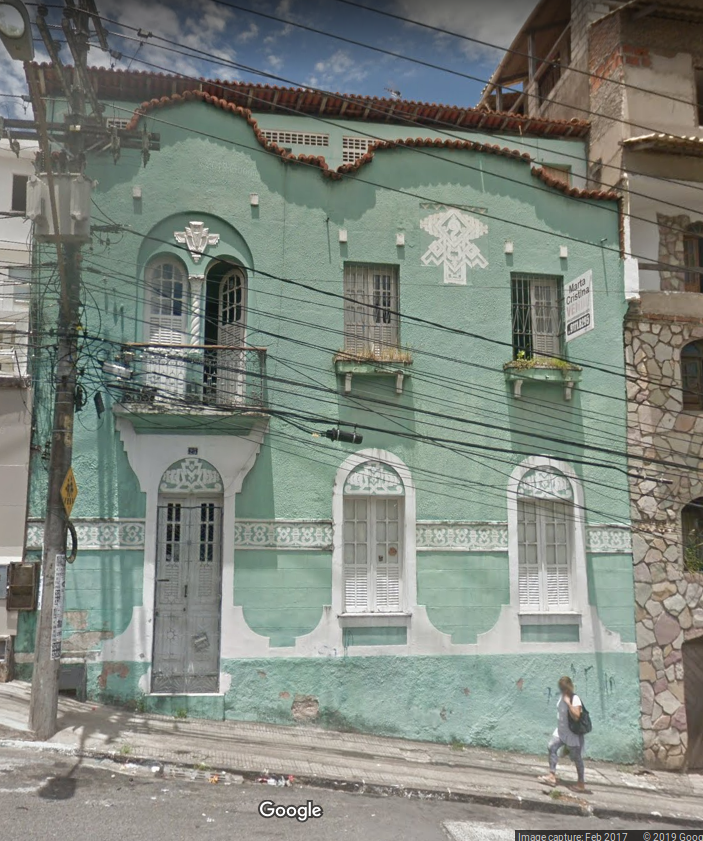
\includegraphics[width=1\textwidth]{8-anexos/plantas/01-1distrito/12-gales/ladeiradosgales-edmundoguimaraes-casa2017.jpg}{\footnotesize \par \textbf{Fonte:} Google Maps. }
\label{fig:edmundoguimaraes2017}
\end{figure}
}